\documentclass[12pt]{article}
\usepackage{geometry}
\geometry{a4paper, margin=1in}
\usepackage{booktabs}
\usepackage{tabularx}
\usepackage{float}
\usepackage{graphicx}
\usepackage{enumitem}
\usepackage{xcolor}
\usepackage{amsmath}
\usepackage{hyperref}
\hypersetup{colorlinks=true, linkcolor=blue, citecolor=blue, urlcolor=blue}

\title{Systems Design Document: Selection of Cryptographic Techniques for the Privacy Preserving Data Analytics Engine (E-Privacy)}
\author{Dilmith D. L. S., Hansana O. G. V., Vidyananda K. H. K.}
\date{September 11, 2026}

\begin{document}
\maketitle

\section{Introduction}
This document identifies the specific cryptographic algorithms, modes, and parameters used to implement each component of the Privacy Preserving Data Analytics Engine (PPDAE) specified in the systems requirements specification. Rather than treating ``encryption'' as a single monolithic control, this design follows the standard three-state model of data protection -- \emph{at rest}, \emph{in transit}, and \emph{in use} -- and selects a distinct, purpose-fit technique for each, since a single cipher cannot satisfy all three simultaneously (in particular, the ``in use'' state requires an additively homomorphic scheme, not a conventional block cipher).

\subsection{Assumptions}
\begin{itemize}[leftmargin=1.5em]
    \item[B1.] All parties (Data Owner client and cloud compute nodes) can execute standard, well-reviewed cryptographic libraries (e.g. OpenSSL, libsodium, python-phe) rather than custom implementations of primitives.
    \item[B2.] The Data Owner's private Paillier key and any symmetric key-encryption keys are generated using a cryptographically secure random number generator (CSPRNG) seeded from the host operating system's entropy source.
    \item[B3.] Clock synchronization (e.g. NTP) is available across components, since signed audit-log entries and TLS session validation depend on reasonably accurate timestamps.
    \item[B4.] The 2048-bit Paillier key length is adopted as the default operating point, per the empirical latency/storage trade-off analysis in Section~\ref{sec:empirical}: it gives an $\sim$11x storage expansion and sub-5-minute aggregation latency for a 2M-record batch, versus 3072-bit's disproportionate latency cost.
    \item[B5.] Where a technique below is described as protecting data ``while in'' a given state, that state boundary corresponds exactly to the trust-domain boundary shown in Figure~\ref{fig:crypto_states}.
\end{itemize}

\section{Cryptographic Techniques by Data State}
Figure~\ref{fig:crypto_states} maps each data-flow segment of the Engine to its assigned cryptographic control.

\begin{figure}[H]
    \centering
    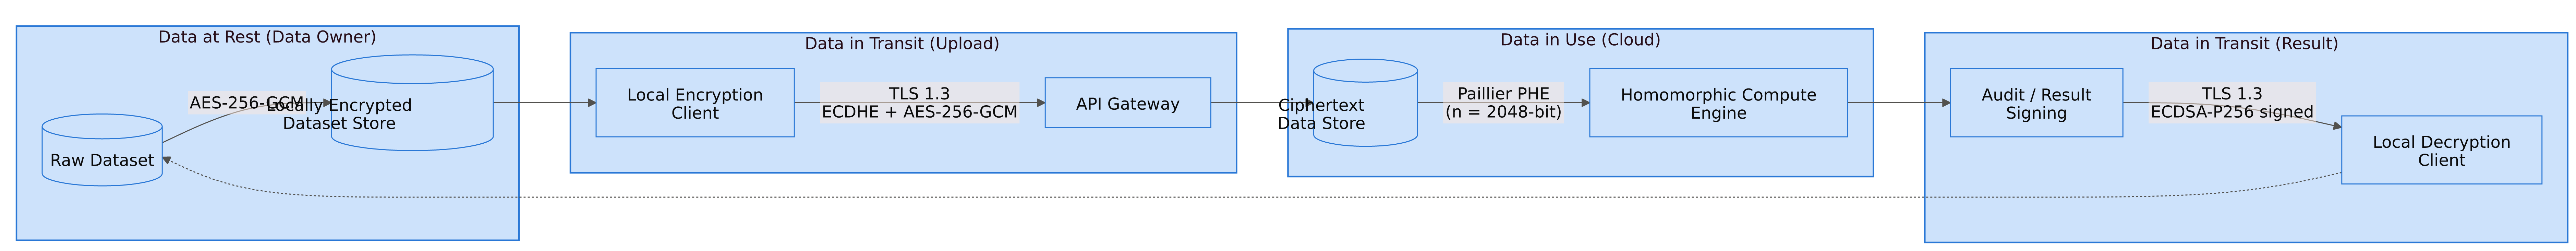
\includegraphics[width=\textwidth]{sources/crypto-design/crypto-per-data-state.png}
    \caption{Cryptographic technique assigned to each data state and transition across the trust boundary.}
    \label{fig:crypto_states}
\end{figure}

\section{Component-Level Cryptographic Specification}

\subsection{Data at Rest (Data Owner's Local Store)}
The raw sensitive dataset, before it is ever homomorphically encrypted for outsourced computation, is protected using the \textbf{AES block cipher with a 256-bit key in GCM mode} (AES-256-GCM) to ensure confidentiality and integrity while the data resides on the Data Owner's local disk. GCM is chosen over CBC because it provides authenticated encryption (confidentiality \emph{and} integrity/tamper-detection) in a single pass, which CBC alone does not. A random 96-bit nonce is generated per encryption operation and never reused with the same key, as required by GCM's security proof.

\subsection{Key Management}
\begin{itemize}[leftmargin=1.5em]
    \item \textbf{Paillier keypair generation:} a probabilistic public/private keypair is generated locally by the Data Owner using two large random primes $p, q$ of equal bit-length, giving a modulus $n = pq$ of the configured length (1024/2048/3072 bits, default 2048 per B4). The public key $(n, g)$ is shared with the cloud engine; the private key $(\lambda, \mu)$ never leaves the Data Owner's trusted domain (per SRS requirement FR-1).
    \item \textbf{Key-encryption key (KEK):} the Paillier private key and the local AES data-encryption key are themselves encrypted at rest under a KEK derived from an administrator passphrase using \textbf{Argon2id} (memory-hard KDF, resistant to GPU/ASIC brute-force), with parameters $t=3$ iterations, $m=64\text{ MiB}$ memory, $p=4$ parallelism lanes.
    \item \textbf{Key rotation:} Paillier keypairs are rotated per analytics campaign (e.g. per reporting quarter); historical ciphertext under a retired key remains decryptable only until that key is securely destroyed, per the organization's data-retention policy.
\end{itemize}

\subsection{Data in Transit}
All network communication between the Data Owner's client and the cloud API Gateway, and between the cloud engine and the client on the return path, uses \textbf{TLS 1.3} with an ECDHE (Elliptic-Curve Diffie--Hellman Ephemeral) key exchange on curve \texttt{X25519} and the \texttt{TLS\_AES\_256\_GCM\_SHA384} cipher suite. TLS 1.3 is selected over 1.2 because it removes legacy negotiable weak cipher suites and mandates forward secrecy for every handshake, so that compromise of a long-term key does not retroactively expose past ciphertext-upload sessions.

\subsection{Data in Use (Homomorphic Computation)}
Aggregation queries (sum, average, count) execute directly over ciphertext using the \textbf{Paillier cryptosystem}, a partially homomorphic public-key scheme with the additive property $E(m_1) \cdot E(m_2) = E(m_1 + m_2) \bmod n^2$ and the affine property $E(m)^k = E(km) \bmod n^2$. This is the only cryptographic control in the design that operates while data is being computed on, which is precisely the ``Data-in-Use'' gap identified as the central architectural flaw of conventional analytics pipelines. Per B4, the default modulus length is \textbf{2048 bits}, giving 112-bit-equivalent security while keeping ciphertext storage and analytics latency within the operational budget established empirically in Section~\ref{sec:empirical}.

\subsection{Access Control and Authentication}
API requests to the Gateway are authenticated using \textbf{JSON Web Tokens (JWT) signed with ECDSA on curve P-256} (ES256). Tokens are short-lived (15-minute expiry) and scoped to a specific role (data ingestion, query submission, audit read) to enforce least privilege. Service-to-service calls between the Gateway and the Homomorphic Compute Engine additionally use \textbf{mutual TLS (mTLS)}, so that only provisioned compute nodes -- not an arbitrary caller holding a valid JWT -- can submit ciphertext for aggregation.

\subsection{Integrity of the Audit / Verifiable Computation Log}
Each entry appended to the Verifiable Computation Log (operation type, input ciphertext hashes, timestamp) is hashed with \textbf{SHA-256} and chained to the previous entry's hash (a hash chain), so that any retroactive edit or deletion is detectable. The chain's current head, together with the computation result, is signed using \textbf{ECDSA-P256}, giving any auditor a way to verify both that the log has not been tampered with and that the signature originates from the legitimate compute engine. This mechanism underpins the individual and universal verifiability properties detailed separately in the verifiability evaluation deliverable.

\section{Empirical Justification of Cryptosystem and Key-Length Selection}
\label{sec:empirical}

To ground the choice of Paillier at a 2048-bit modulus (assumption B4 and the ``Data in Use'' specification above) in evidence rather than assertion, the Feasibility and Computation Overhead studies benchmarked four candidate approaches -- \textbf{Plaintext} (baseline), \textbf{RSA} (decrypt-compute-re-encrypt), \textbf{PHE / Paillier} (additive homomorphism), and \textbf{FHE / TenSEAL CKKS} (arbitrary homomorphism) -- across key lengths of 1024, 2048, and 3072 bits, extrapolated from a 1{,}000-record sample to a full 2{,}000{,}000-record / 94.76~MB financial dataset (a 2000x scale factor).

\subsection{Storage Footprint}
Figure~\ref{fig:storage} shows that FHE ciphertext expansion is catastrophic for tabular aggregation workloads (up to 617~GB for a 94.76~MB source file, a $\sim$6{,}600x expansion), while PHE remains within a manageable $\sim$11--16x expansion across all tested key lengths.

\begin{figure}[H]
    \centering
    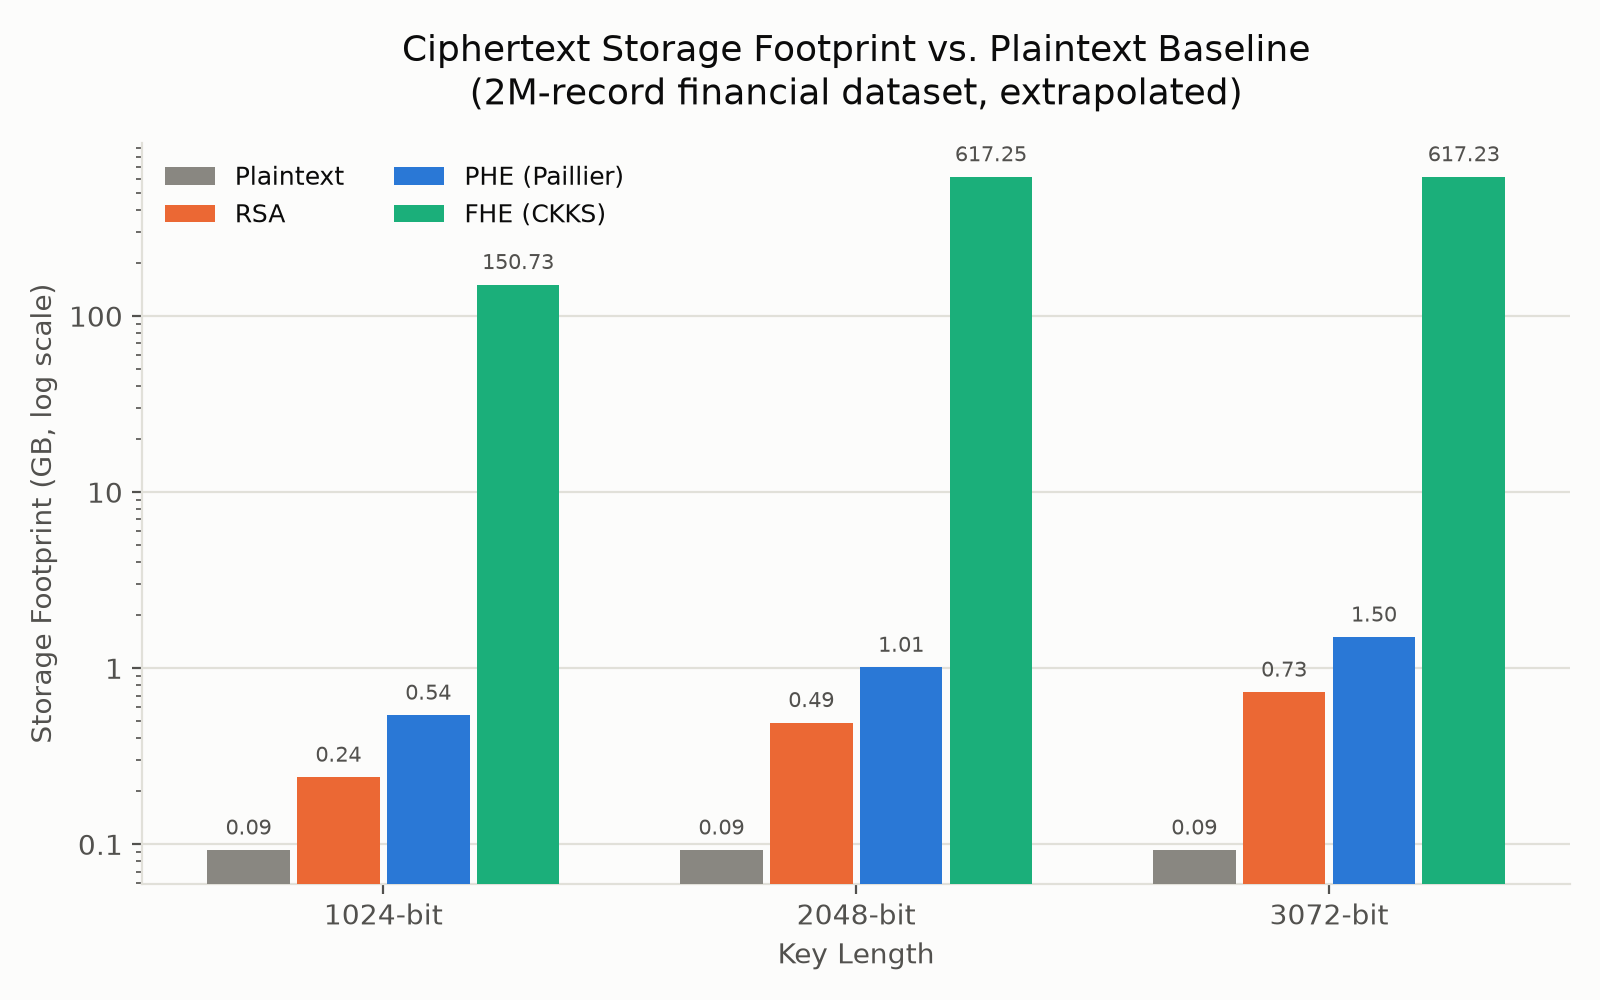
\includegraphics[width=0.85\textwidth]{sources/crypto-design/chart-storage-footprint.png}
    \caption{Ciphertext storage footprint by cryptographic scheme and key length (log scale).}
    \label{fig:storage}
\end{figure}

\subsection{Encryption Latency}
Figure~\ref{fig:enc_latency} shows the full-dataset encryption latency. PHE encryption is the slowest to \emph{ingest} at higher key lengths (112 hours at 3072-bit), which is why the default configuration (B4) targets 2048-bit keys and a parallelized/pipelined ingestion process rather than blocking on full-dataset encryption before any query can run.

\begin{figure}[H]
    \centering
    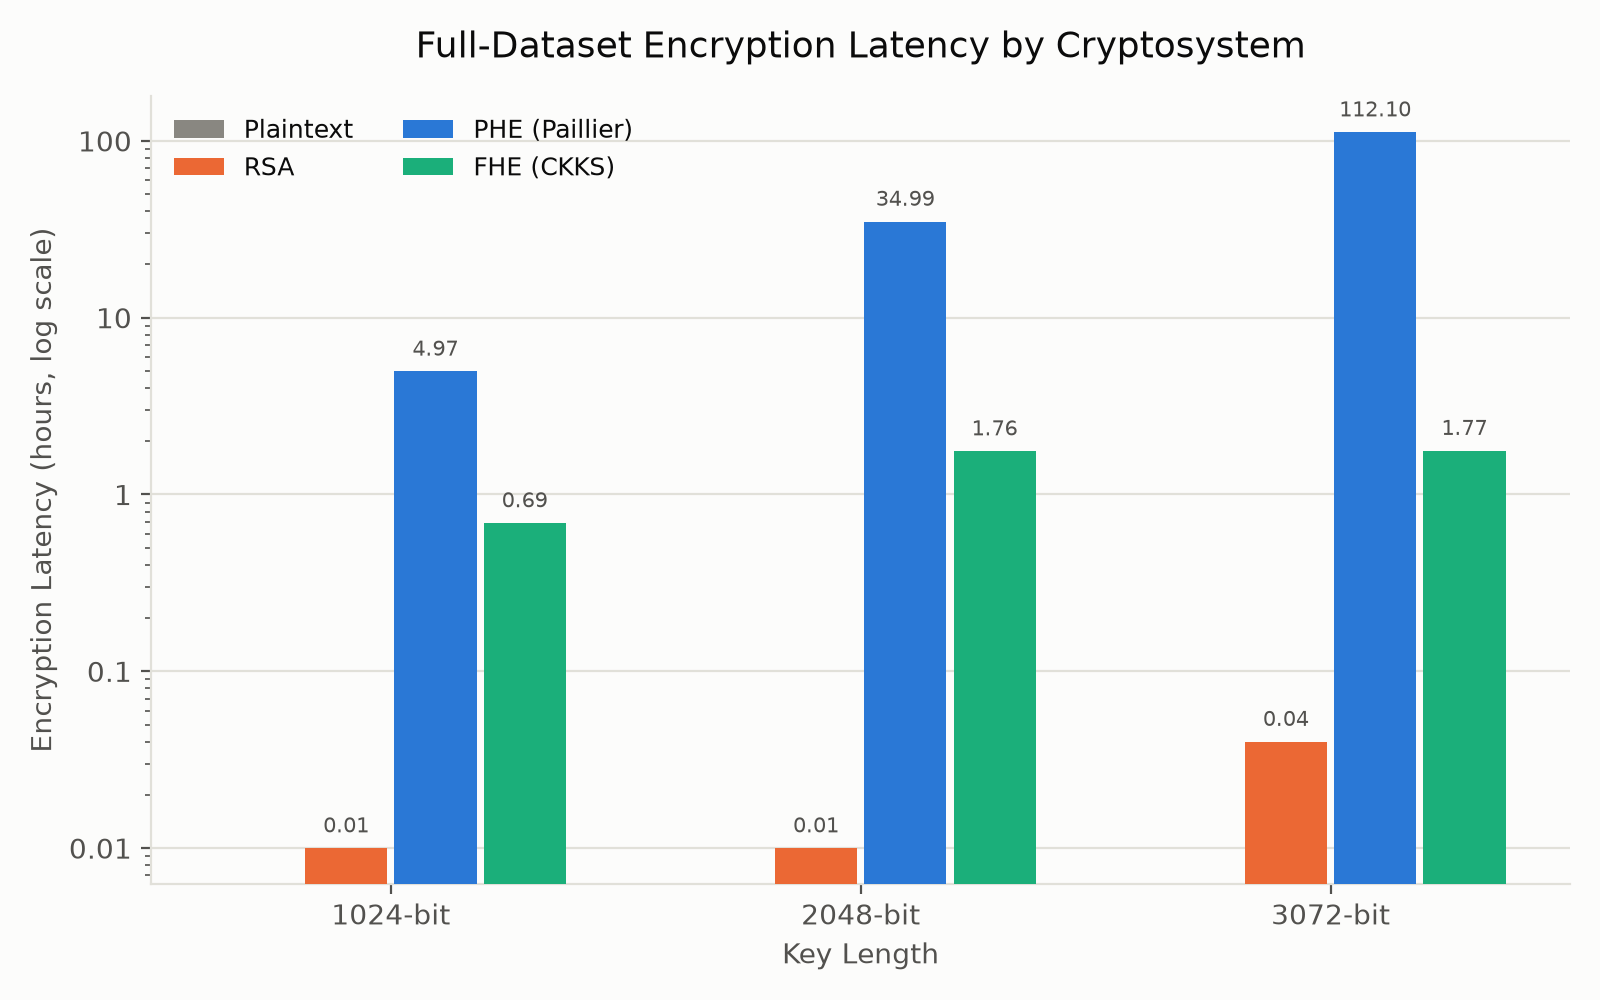
\includegraphics[width=0.85\textwidth]{sources/crypto-design/chart-encryption-latency.png}
    \caption{Full-dataset encryption latency by cryptographic scheme and key length (log scale).}
    \label{fig:enc_latency}
\end{figure}

\subsection{Analytics (Query) Latency}
Figure~\ref{fig:analytics_latency} shows the latency of the actual sum/average computation on already-encrypted data -- the metric that dominates user-perceived query responsiveness. PHE outperforms both RSA's decrypt-compute-re-encrypt pipeline (which additionally violates the Data-in-Use confidentiality requirement, since it requires server-side plaintext exposure) and FHE at every key length tested.

\begin{figure}[H]
    \centering
    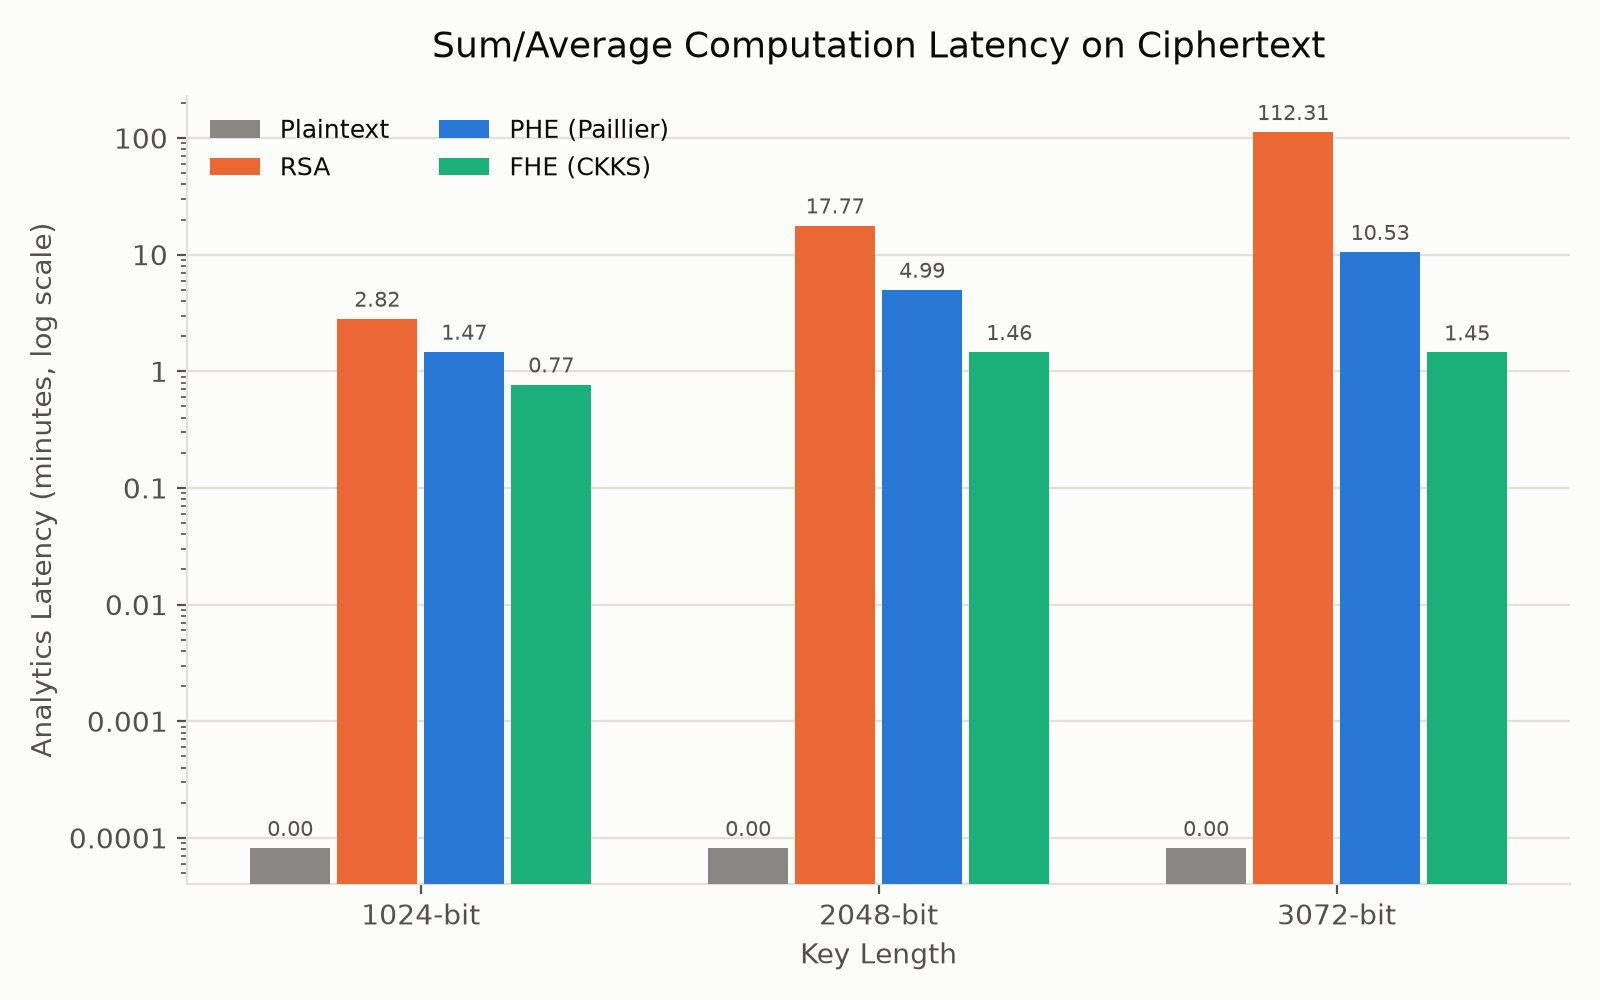
\includegraphics[width=0.85\textwidth]{sources/crypto-design/chart-analytics-latency.png}
    \caption{Ciphertext sum/average computation latency by cryptographic scheme and key length (log scale).}
    \label{fig:analytics_latency}
\end{figure}

\subsection{Trade-off Synthesis}
Figure~\ref{fig:tradeoff} plots storage footprint against analytics latency for the three encrypted schemes. PHE occupies the most favorable region of the trade-off space -- low storage expansion \emph{and} low query latency -- for additive aggregation workloads, whereas FHE's generality is paid for with orders-of-magnitude worse storage and no corresponding analytics-latency benefit for this workload class.

\begin{figure}[H]
    \centering
    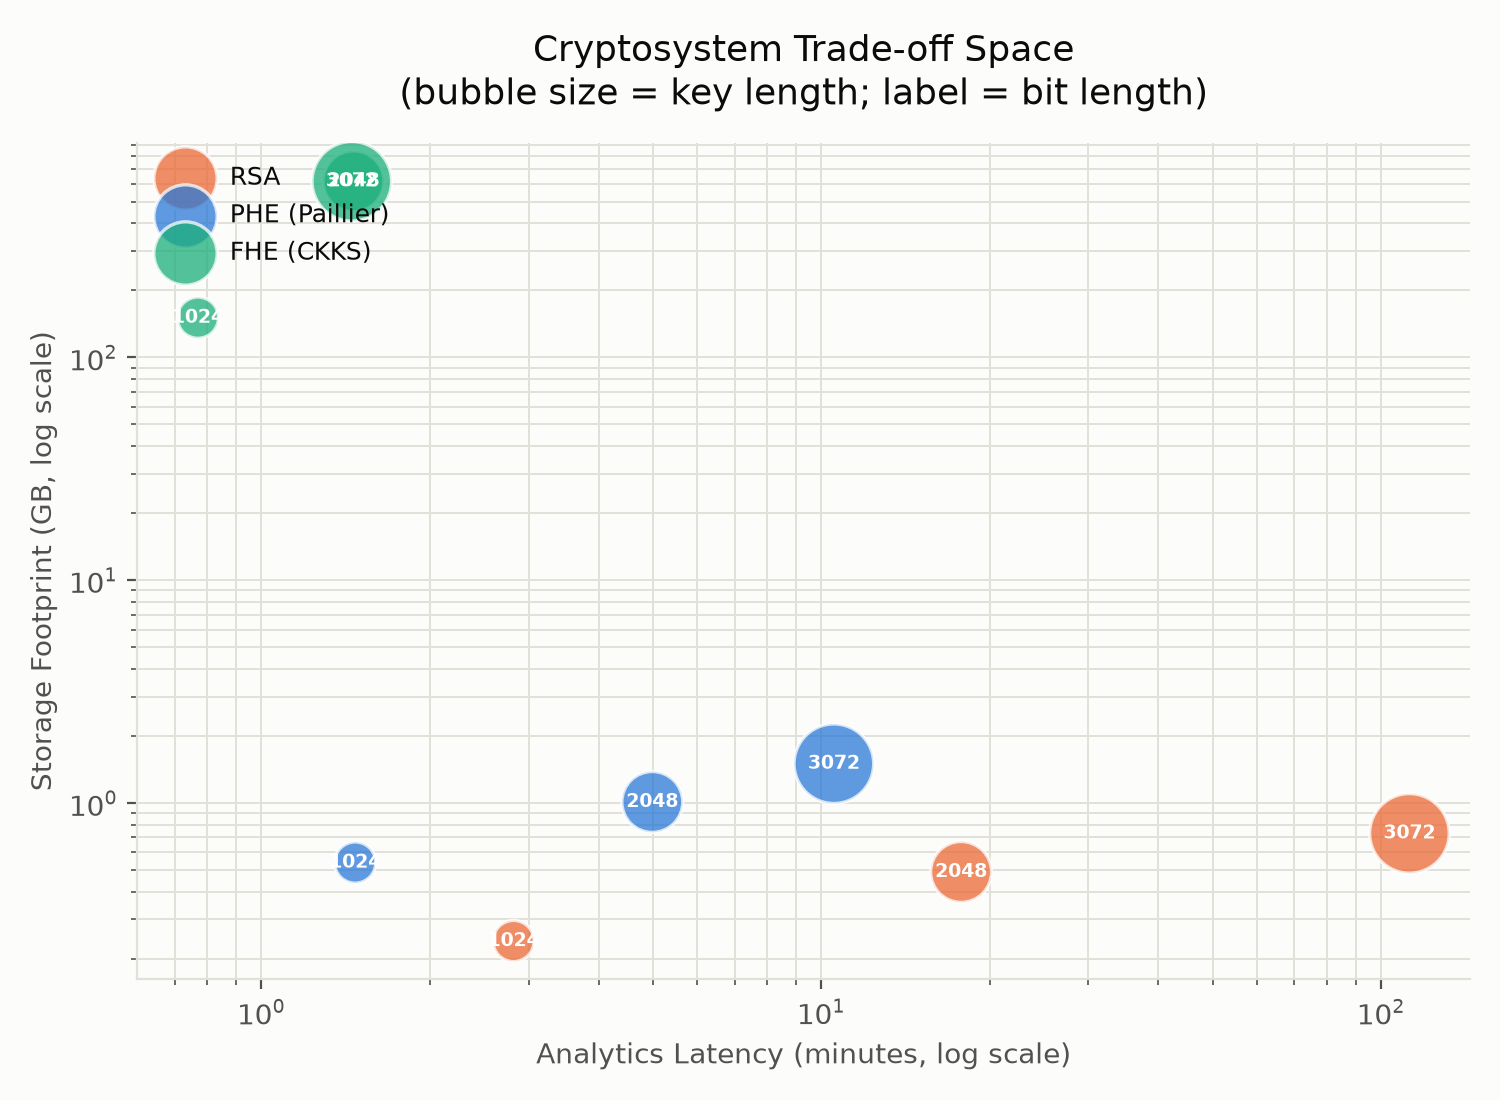
\includegraphics[width=0.8\textwidth]{sources/crypto-design/chart-tradeoff-scatter.png}
    \caption{Storage footprint vs. analytics latency trade-off space across cryptosystems and key lengths.}
    \label{fig:tradeoff}
\end{figure}

\subsection{Decision}
Based on this empirical evidence, the Homomorphic Computation Engine is specified around Partially Homomorphic Encryption (Paillier) at a default 2048-bit key length, matching the industry-standard security margin while keeping storage expansion and analytics latency within operationally acceptable bounds. FHE (CKKS) is retained as a \emph{pluggable future option} for workloads that require multiplicative operations between two ciphertexts, which Paillier does not support.

\section{Summary of Cryptographic Parameters}

\begin{table}[H]
\centering
\begin{tabularx}{\textwidth}{l l l X}
\toprule
\textbf{Component} & \textbf{Technique} & \textbf{Parameters} & \textbf{Purpose} \\
\midrule
Local dataset store & AES-GCM & 256-bit key, 96-bit nonce & Confidentiality \& integrity of data at rest \\
KEK derivation & Argon2id & $t{=}3$, $m{=}64$ MiB, $p{=}4$ & Protect stored key material from offline brute-force \\
Network transport & TLS 1.3 (ECDHE X25519) & \texttt{TLS\_AES\_256\_GCM\_SHA384} & Confidentiality \& integrity of data in transit; forward secrecy \\
Homomorphic aggregation & Paillier (PHE) & $n$ = 2048-bit modulus & Confidentiality of data in use; enables additive computation without decryption \\
API authentication & JWT (ES256) & 15-min expiry, scoped claims & Access control / least privilege \\
Service-to-service auth & mutual TLS & X.509 client certs & Restrict ciphertext submission to provisioned compute nodes \\
Audit log & SHA-256 hash chain + ECDSA-P256 signature & 256-bit hash, P-256 curve & Tamper-evidence and verifiability of computation history \\
\bottomrule
\end{tabularx}
\caption{Cryptographic techniques and parameters by component.}
\label{tab:crypto_summary}
\end{table}

\section{Conclusion}
No single cryptographic primitive can secure the Engine end-to-end: symmetric AES-GCM protects data at rest, TLS 1.3 protects data in transit, and only an additively homomorphic scheme -- Paillier at a 2048-bit modulus -- can protect data while it is being computed on, which is the property that distinguishes this design from conventional analytics platforms. JWT-based access control, mutual TLS, and a signed hash-chained audit log together provide the authentication and integrity controls needed to make the resulting computations trustworthy and auditable.

\end{document}
